\section*{3. Heun's Method --- 2nd-Order Sampler (EC3)}

\subsection*{Problem \& Approach}
\textbf{Main HW3 samples with Euler integration} ($T=100$ steps, constant $\Delta t = 1/T$). EC3 asks whether a 2nd-order Heun sampler improves on that integrator without retraining. We use the same x-prediction model (main HW3 configuration) and compare Heun ($N$ steps) vs.\ Euler ($2N$ steps) at equal function evaluations (NFE), following Karras et al.\ (2022).

Main HW3 also showed (Viz 2c) that sample quality degrades with fewer Euler steps. EC3 extends that analysis with a higher-order integrator.

\begin{figure}[h]
    \centering
    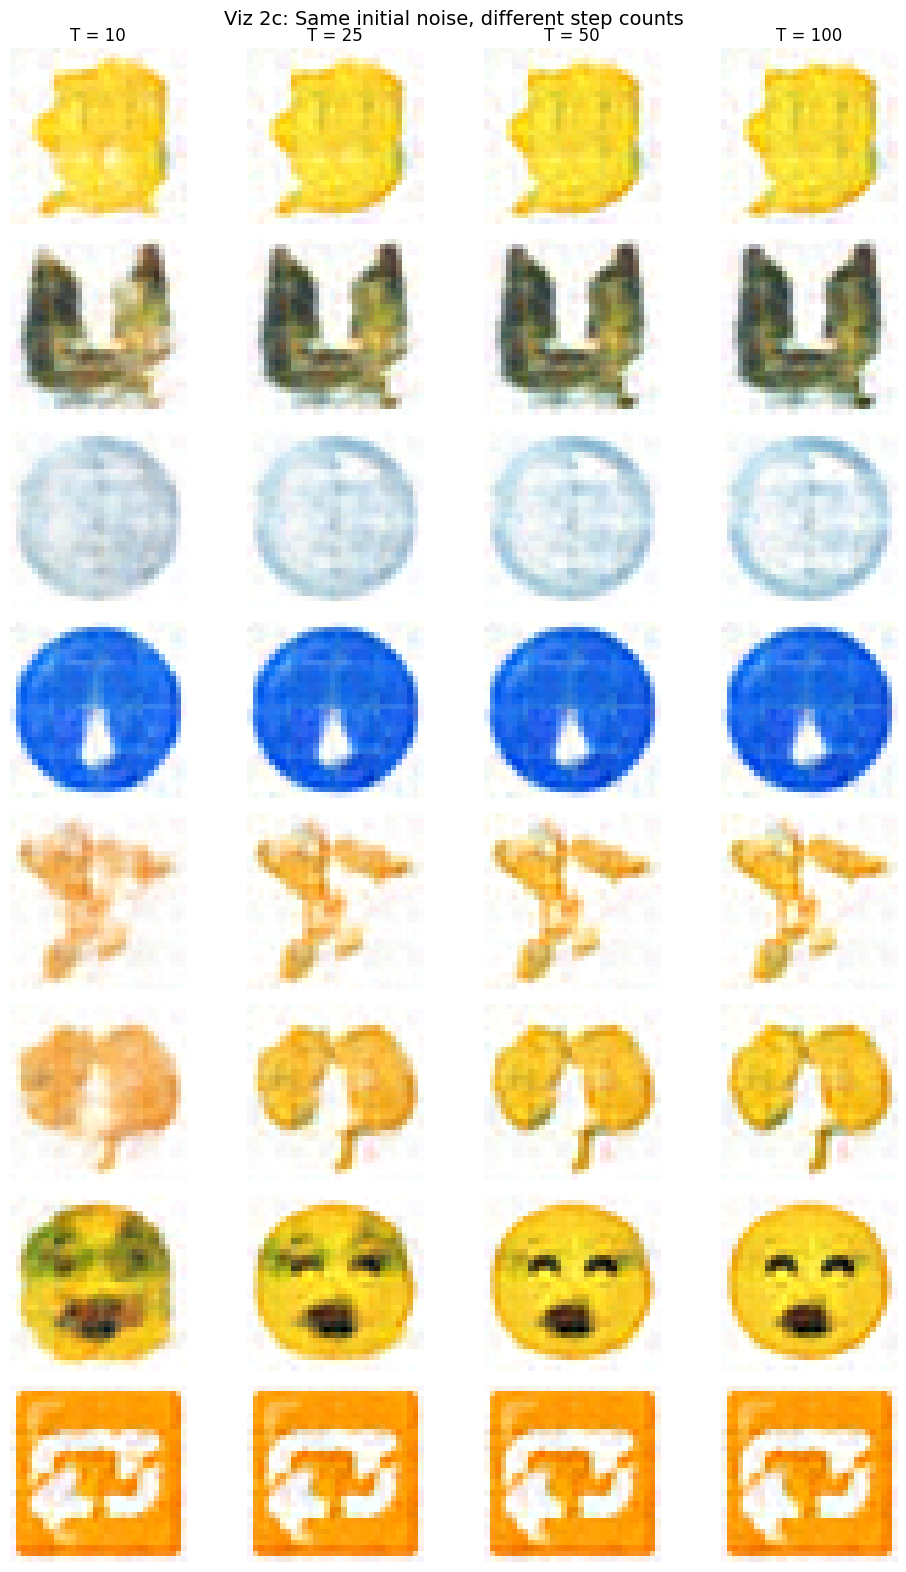
\includegraphics[width=0.75\textwidth]{figures/hw3_main_steps.png}
    \caption{Main HW3: same noise, Euler at $T \in \{10, 25, 50, 100\}$. EC3 improves on this Euler baseline.}
    \label{fig:main_steps}
\end{figure}

\subsection*{Results}

\begin{table}[h]
\centering
\begin{tabular}{l c c l}
\toprule
\textbf{NFE Budget} & \textbf{Heun (L2 to ref)} & \textbf{Euler (L2 to ref)} & \textbf{Main HW3 uses} \\
\midrule
10 & 12.593 & 12.904 & Euler $T{=}10$ \\
20 & 8.658 & 9.299 & --- \\
50 & 4.894 & 5.028 & Euler $T{=}50$ \\
100 & --- & --- & Euler $T{=}100$ (default) \\
\bottomrule
\end{tabular}
\caption{Discretization error vs.\ a $T=200$ Euler reference (lower $=$ better). Main HW3's default is Euler $T=100$.}
\label{tab:ec3_nfe}
\end{table}

\begin{figure}[h]
    \centering
    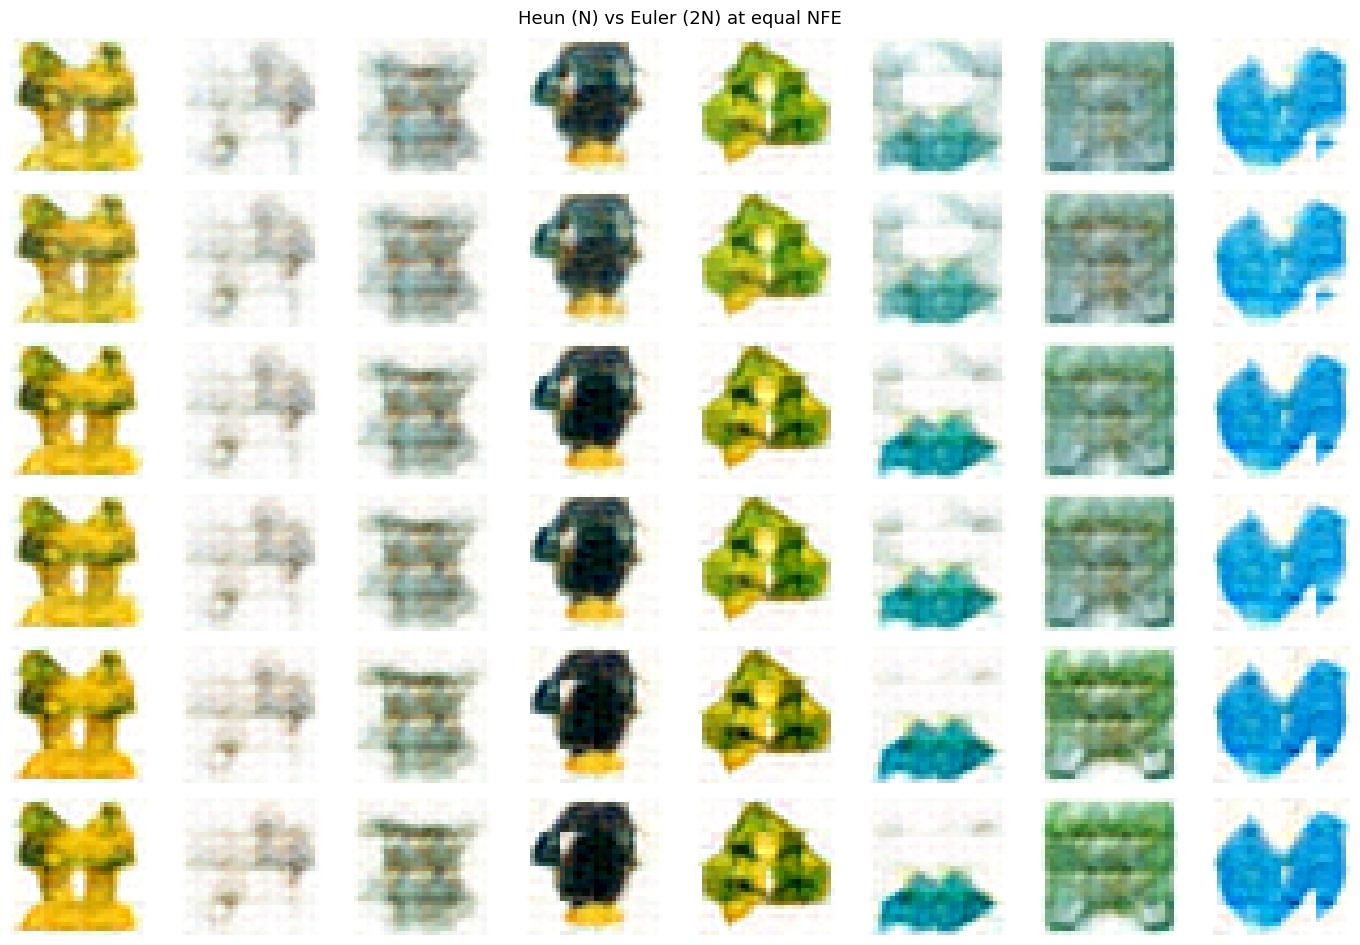
\includegraphics[width=0.95\textwidth]{figures/ec3_heun_vs_euler.png}
    \caption{Heun ($N$) vs.\ Euler ($2N$) at equal NFE---direct improvement over main HW3's integrator.}
    \label{fig:ec3_grid}
\end{figure}

\begin{figure}[h]
    \centering
    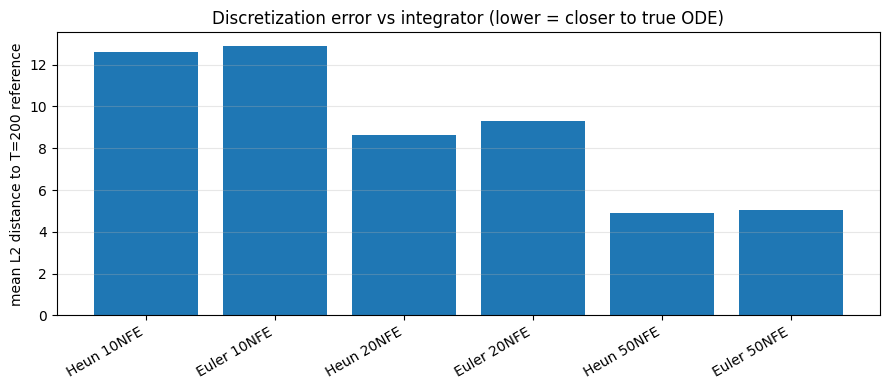
\includegraphics[width=0.65\textwidth]{figures/ec3_nfe_bar.png}
    \caption{Heun consistently closer to the true ODE solution than Euler at matched NFE.}
    \label{fig:ec3_bar}
\end{figure}

\subsection*{Discussion}
Heun improves on main HW3's Euler sampler at every tested NFE budget (2--3\% lower discretization error). The gain is largest at low budgets---where main HW3's Viz 2c showed visible quality loss---and narrows at 50 NFE. For main HW3's default $T=100$, Heun with $T=50$ would match NFE while likely producing sharper samples. Flow matching's straight trajectories mean Euler is already decent at $T=100$; Heun is most valuable when sampling cost is constrained.
